\documentclass[12pt,a4paper, blue]{bbe}
\usepackage{blindtext}
\usepackage{listings}
\usepackage{xcolor}
\usepackage{subfiles}
\usepackage{hyperref} %for Hyperlinks

\definecolor{codegreen}{rgb}{0,0.6,0}
\definecolor{codegray}{rgb}{0.5,0.5,0.5}
\definecolor{codepurple}{rgb}{0.58,0,0.82}
\definecolor{codebackcolour}{rgb}{0.95,0.95,0.92}

  	
%added be me.
%Code listing style named "mystyle"
\lstdefinestyle{mystyle}{
    backgroundcolor=\color{codebackcolour},
    commentstyle=\color{codegreen},
    keywordstyle=\color{magenta},
    numberstyle=\tiny\color{codegray},
    stringstyle=\color{codepurple},
    basicstyle=\ttfamily\footnotesize,
    breakatwhitespace=false,         
    breaklines=true,                 
    captionpos=b,                    
    keepspaces=true,                 
    numbers=left,                    
    numbersep=5pt,                  
    showspaces=false,                
    showstringspaces=false,
    showtabs=false,                  
    tabsize=2
}

\lstset{style=mystyle}

\begin{document}

	\chapter{Setting up}
	
	\section{Getting up an running with python}
	
	Initially to get going with python and have fun coding you could use an online editor. I recommend Google colab. This is an online notebook where you can run python in your browser and also make notes at the same time.
	\vspace{1cm}
	
	\begin{figure}[h]
        \centering
        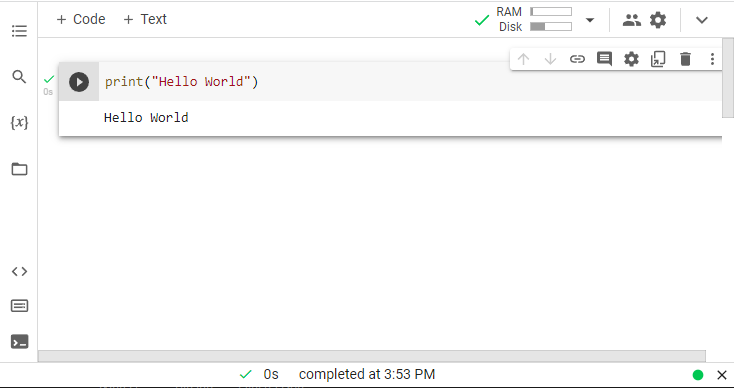
\includegraphics[width=0.8\textwidth]{images/ch1/colab1.PNG}
        \caption{Google colab online}
        \label{fig:mesh1}
    \end{figure}
    \vspace{5mm}
    
    Shown above in Figure 1.1 is the web interface for google colab. This shows a code pane where you can enter code and then use the play button to run the code live in the browser. You can have several blocks of code if you wish. The text block is handy to make notes - as shown below in F1.2
	\vspace{1cm}
	\begin{figure}[h]
        \centering
        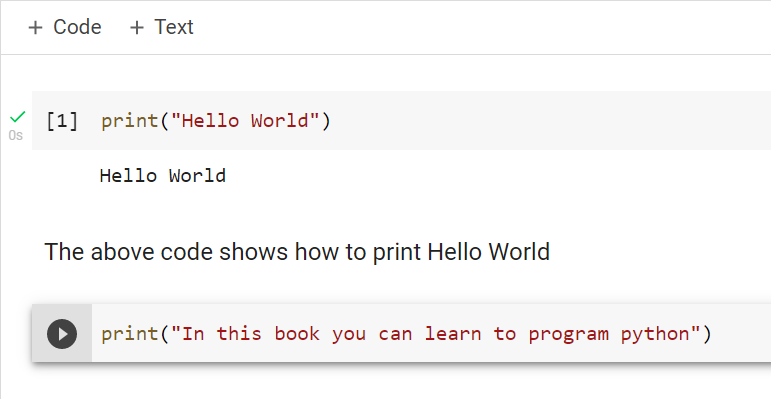
\includegraphics[width=0.8\textwidth]{images/ch1/colab2.PNG}
        \caption{Google colab online}
        
    \end{figure}
	
	
	\begin{link}[]
    	\begin{itemize}[c]     % see bbe 653
    	    \item Google Colab   \url{https://colab.research.google.com/}
    	    \item RPEL it
    	    \item Jupyter notebook
	    \end{itemize}
	
	\end{link}
	
	
	\section{Lets start coding!}
	
	It is customary to start with 'Hello World' to learn how to print out words.
	

	\begin{lstlisting}
    print("Hello World")\end{lstlisting}
	
    After running this with the > button it should print Hello World
    
    \begin{lstlisting}
    > Hello World\end{lstlisting}
    
    
    
    \section{Using Variables}
    
    When making computer program we will have to store information so that it can be used or changed.
    Variables - also called identifiers are used to store data of different types.
    
    \vspace{5mm}
    \textbf{Integers - Whole numbers}
    
    \begin{lstlisting}
    age = 18
    score = 50
    counter = 400\end{lstlisting}
    
    try and make a few yourself.
    
    We can print out the stored variables. Make a new box in colab by pressing the +Code button
    
    \begin{lstlisting}
    print(age)
    print(score)
    print(counter)\end{lstlisting}
    
    This will output the following:
    \begin{lstlisting}
    > 18
    > 50
    > 400\end{lstlisting}
    
    
    \vspace{5mm}
    \textbf{Float - Floating point - decimal numbers}
    \begin{lstlisting}
    money =  8.25
    pi = 3.142
    gravity = 9.8\end{lstlisting}
    Floating point numbers can be used to store numerical data with more accuracy than a whole number. Useful for representing money, or other numbers where accuracy is needed. In some languages you have to specifically state that a number is of type - float, but in python the run-time compiler takes care of this for you. 
    
    \begin{remark}
	Have a go at making your own a printing out your floats.
	\end{remark}
    
    \vspace{5mm}
    \textbf{Strings - Text, words, letters}
    \begin{lstlisting}
    name =  "Paul"
    codeword = "abc123"
    day = "Wednesday
    phone = "01234 5678920\end{lstlisting}
    Sting data is used for text, and also for mixing numbers and letters. If calculations are not needed string information can be used for some numbers - such as a phone number as this will allow you to have spaces and leading zero's
    
    \vspace{5mm}
    \textbf{Boolean - True or false values}
    \begin{lstlisting}
    raining = False
    valid = True
    \end{lstlisting}
    A boolean value represent a true or false state. For instance a value may represent the state of something in your program such as if an option is selected or not. 
    
    
	\begin{recap}
	\begin{itemize}
	    \item Integer - Whole number
	    \item Float -  Decimal or fractional number
	    \item String - Words/text
	    \item Boolean -  True or False value
	\end{itemize}
	These data types are used to store information and can also be used in calculations. Choosing the correct data type is important for your program to work correctly. Python will crash if trying to add a number and a string!
	\end{recap}
	

	
\end{document}

